\documentclass[letterpaper,12pt]{article}
\usepackage{tabularx} % extra features for tabular environment
\usepackage{amsmath}  % improve math presentation
\usepackage{graphicx} % takes care of graphic including machinery
\usepackage[margin=1in,letterpaper]{geometry} % decreases margins
\usepackage{cite} % takes care of citations
\usepackage{longtable}
\usepackage{booktabs}
\usepackage[final]{hyperref} % adds hyper links inside the generated pdf file
\hypersetup{
	colorlinks=true,       % false: boxed links; true: colored links
	linkcolor=blue,        % color of internal links
	citecolor=blue,        % color of links to bibliography
	filecolor=magenta,     % color of file links
	urlcolor=blue         
}
\usepackage{blindtext}
%++++++++++++++++++++++++++++++++++++++++


\begin{document}

\title{Predict Active Regulatory Regions Using Deep Learning Models in HEK293 cell line}
\author{Michele Antonazzi}
\date{\today}
\maketitle

\begin{abstract}
In this work, we studied the prediction of active and inactive regulatory regions (promoters and enhancers) in the HEK293 cell line. 
The aim is to prove the effectiveness of deep learning models using both epigenomic and sequence data. In particular, the deep models tested are feed-forward neural network (FFNN) and convolutional neural networks (CNN), which are used on the epigenomic and sequence data respectively.
\end{abstract}

\input{introduction.tex}
\newpage

\section{Models}

This project aims to predict if regulatory elements, such as promoters
and enhancers, are active or inactive in a specific cell line using
supervised deep learning methods. More precisely, the tasks are two:
predict the activity or inactivity of the promoters and predict the
activity or inactivity of enhancers in a specific cell line, the HEK293.
As mentioned in the introduction, the DNA is the same in all the cells
of an organism but the gene expression changes according to the cell
type and its function. This process, which is really complex and largely
still unknown, is heavily influenced by the activity of the CREs.
However, locate the active DNA region is a very complex and expensive
task in Biology and Computer Science can help to predict active
regulatory elements using features that characterize them. The type of
data related to the regulatory region (promoters and enhancers) are two:
the epigenomic and sequence data. The two tasks described before (to
distinguish active and inactive enhancers and promoters) are performed
using both epigenomic and sequence data. To do this, supervised machine
learning methods are used. In particular, given the diversity of the two
types of data, two different models are used in his project: FFNN
(feedforward neural network) and CNN (convolutional neural network),
respectively for epigenomic and sequence data. These models are very
complicated, not easy to set up, and computationally hard to execute. To
verify the performance of these models, their results are compared with
those of simpler learning machines: decision tree, random forest,
perceptron, and multilayer perceptron (MLP).

\subsection{FFNN}

The feed-forward neural networks are used to analyze the epigenomic data
related to promoters and enhancers. Each region is characterized by a
lot of features, about 200, so the data have high dimensionality. An
FFNN is suitable for processing these data using more layers and
neurons. In particular, in this project, three different types of FFNN
are tested. The first model (called FFNN\_1) has a classical
architecture and it is set using almost standard parameters. Its purpose
is to examine the network performance with the given dataset to build a
better model.

\begin{longtable}[]{@{}lllll@{}}
\toprule
\textbf{Layers} & \textbf{Type} & \textbf{Units} & \textbf{Activation} & \textbf{Probability}\tabularnewline
\midrule
\endhead
Layer 1 & Dense & 256 & ReLU & -\tabularnewline
Layer 2 & Dense & 128 & ReLU & -\tabularnewline
Layer 3 & Batch Normalization & - & ReLU & -\tabularnewline
Layer 4 & Dense & 64 & ReLU & -\tabularnewline
Layer 5 & Dropout & - & - & 0.3\tabularnewline
Layer 6 & Dense & 32 & ReLU & -\tabularnewline
Layer 7 & Dense & 16 & ReLU & -\tabularnewline
Layer 8 & Dense & 1 & Sigmoid & -\tabularnewline
\bottomrule
\end{longtable}

\begin{longtable}[]{@{}ll@{}}
\toprule
\textbf{Parameter} & \textbf{Value}\tabularnewline
\midrule
\endhead
Weight estimator & nadam\tabularnewline
Learning rate & 0.001\tabularnewline
Loss function & binary crossentropy\tabularnewline
Epochs & 1000\tabularnewline
Batch size & 1024\tabularnewline
Validation split & 0.1\tabularnewline
Shuffle & true\tabularnewline
Early stopping & monitor = val\_loss, patience = 50\tabularnewline
\bottomrule
\end{longtable}

The second feedforward neural network (FFNN\_2) is similar to the first:
it has only more Dropout layers with a higher rate to prevent
overfitting.

\begin{longtable}[]{@{}lllll@{}}
\toprule
\textbf{Layers} & \textbf{Type} & \textbf{Units} & \textbf{Activation} & \textbf{Probability}\tabularnewline
\midrule
\endhead
Layer 1 & Dense & 256 & ReLU & -\tabularnewline
Layer 2 & Dropout & - & - & 0.5\tabularnewline
Layer 3 & Batch Normalization & - & ReLU & -\tabularnewline
Layer 4 & Dense & 128 & ReLU & -\tabularnewline
Layer 5 & Dropout & - & - & 0.5\tabularnewline
Layer 6 & Dense & 64 & ReLU & -\tabularnewline
Layer 7 & Dropout & - & - & 0.5\tabularnewline
Layer 8 & Dense & 32 & ReLU & -\tabularnewline
Layer 9 & Dropout & - & - & 0.5\tabularnewline
Layer 10 & Dense & 16 & ReLU & -\tabularnewline
Layer 11 & Dropout & - & - & 0.5\tabularnewline
Layer 12 & Dense & 1 & Sigmoid & -\tabularnewline
\bottomrule
\end{longtable}

\begin{longtable}[]{@{}ll@{}}
\toprule
\textbf{Parameter} & \textbf{Value}\tabularnewline
\midrule
\endhead
Weight estimator & nadam\tabularnewline
Learning rate & 0.001\tabularnewline
Loss function & binary crossentropy\tabularnewline
Epochs & 1000\tabularnewline
Batch size & 1024\tabularnewline
Validation split & 0.1\tabularnewline
Shuffle & true\tabularnewline
Early stopping & monitor = val\_loss, patience = 50\tabularnewline
\bottomrule
\end{longtable}

\newpage
The third learning machine (FFNN\_3) tries to resolve the problem of
data imbalance. First of all, a bias is added to the last layer to
reflect the class imbalance. Then, a particular parameter that specifies
the class weight is passed for the learning procedure. This solution is
taken from this official Tensorflow \href{https://www.tensorflow.org/tutorials/structured_data/imbalanced_data}{guide}.
In this network is also set a different early stopping condition, which
maximizes the AUPRC and restores the best weights after each epoch.

\begin{longtable}[]{@{}llllll@{}}
\toprule
\textbf{Layers} & \textbf{Type} & \textbf{Units} & \textbf{Activation} & \textbf{Probability} & \textbf{Notes}\tabularnewline
\midrule
\endhead
Layer 1 & Dense & 256 & ReLU & - & -\tabularnewline
Layer 2 & Batch Normalization & - & ReLU & - & -\tabularnewline
Layer 3 & Dense & 128 & ReLU & - & -\tabularnewline
Layer 4 & Dense & 64 & ReLU & - & -\tabularnewline
Layer 5 & Dense & 32 & ReLU & - & -\tabularnewline
Layer 6 & Dropout & - & - & 0.5 & -\tabularnewline
Layer 7 & Dense & 16 & ReLU & - & -\tabularnewline
Layer 8 & Dropout & - & - & 0.5 & -\tabularnewline
Layer 9 & Dense & 1 & Sigmoid & - & bias initializer\tabularnewline
\bottomrule
\end{longtable}

\begin{longtable}[]{@{}ll@{}}
\toprule
\textbf{Parameter} & \textbf{Value}\tabularnewline
\midrule
\endhead
Weight estimator & nadam\tabularnewline
Learning rate & 0.001\tabularnewline
Loss function & binary crossentropy\tabularnewline
Epochs & 1000\tabularnewline
Batch size & 1024\tabularnewline
Validation split & 0.1\tabularnewline
Shuffle & true\tabularnewline
Early stopping & monitor = val\emph{aurpc, patience = 50,
restore}best\_weight = true\tabularnewline
Class weight & dictionary with class weight\tabularnewline
\bottomrule
\end{longtable}

The last model type (FFNN\_4) is inspired by Bayesian-FFNN explained in
{[}5{]}, constructed using the Bayesian optimization method. Its
architecture is composed of 3 hidden layers with an l2 regularizer,
which apply a penalty on the layer's kernel.

\begin{longtable}[]{@{}lllll@{}}
\toprule
\textbf{Layers} &\textbf{Type} & \textbf{Units} & \textbf{Activation} & \textbf{Regularizer l2}\tabularnewline
\midrule
\endhead
Layer 1 & Dense & 256 & ReLU & 0.001\tabularnewline
Layer 3 & Dense & 128 & ReLU & 0.001\tabularnewline
Layer 4 & Dense & 64 & ReLU & 0.001\tabularnewline
Layer 8 & Dense & 1 & Sigmoid & -\tabularnewline
\bottomrule
\end{longtable}

\newpage
\begin{longtable}[]{@{}ll@{}}
\toprule
\textbf{Parameter} & \textbf{Value}\tabularnewline
\midrule
\endhead
Weight estimator & SGD\tabularnewline
Learning rate & 0.1\tabularnewline
learning rate decay & 0.01\tabularnewline
Loss function & binary crossentropy\tabularnewline
Epochs & 1000\tabularnewline
Batch size & 100\tabularnewline
Validation split & 0.1\tabularnewline
Shuffle & true\tabularnewline
Early stopping & monitor = val\_loss, patience = 50\tabularnewline
\bottomrule
\end{longtable}

\subsection{CNN}\label{header-n371}

The convolutional neural networks are used to analyze the sequence data
because they can find patterns or motives which characterize this type
of data. In the sequence data the features are hidden inside the
sequence itself, so a CNN at first learns what are the data features
using convolutional layers and subsequently uses these features to label
the data thanks to fully connected layers. A feed-forward neural network
uses only nucleotide locations as functionality but this information is
too weak to effectively classify data. In this project are build and
tested three different CNNs. The first network (CNN\_1) is used to
evaluate the performance of the network using the data related to the
HEK293 cell line.

\begin{longtable}[]{@{}llllll@{}}
\toprule
\textbf{No. of Layers} & \textbf{Type} & \textbf{Units} & \textbf{Kernel size} & \textbf{Activation} &
\textbf{Notes}\tabularnewline
\midrule
\endhead
1 & Reshape & - & - & - & shape = 200, 4, 1\tabularnewline
2 & Conv2D & 64 & 10, 2 & ReLU & -\tabularnewline
1 & Dropout & - & - & - & Probability = 0.3\tabularnewline
1 & Conv2D & 32 & 10, 2 & ReLU & strides = 2, 1\tabularnewline
2 & Conv2D & 32 & 10, 1 & ReLU & -\tabularnewline
1 & Dropout & - & - & - & Probability = 0.3\tabularnewline
1 & Flatten & - & - & - & -\tabularnewline
1 & Dense & 32 & - & ReLU & -\tabularnewline
1 & Dense & 16 & - & ReLU & -\tabularnewline
1 & Dense & 1 & - & Sigmoid & -\tabularnewline
\bottomrule
\end{longtable}

\begin{longtable}[]{@{}ll@{}}
\toprule
\textbf{Parameter} & \textbf{Value}\tabularnewline
\midrule
\endhead
Weight estimator & nadam\tabularnewline
Learning rate & 0.001\tabularnewline
Loss function & binary crossentropy\tabularnewline
Epochs & 100\tabularnewline
Batch size & 1024\tabularnewline
Shuffle & true\tabularnewline
\bottomrule
\end{longtable}

The second network (CNN\_2) has a different architecture. In particular,
the convolutional layers have a larger unit number, to better find the
patterns and features which characterized the data, and they apply a
stride to reduce the parameter number. Besides, the dropout related to
the fully-connected layer is increased to reduce overfitting.

\begin{longtable}[]{@{}llllll@{}}
\toprule
\textbf{No. of Layers} & \textbf{Type} & \textbf{Units} & \textbf{Kernel size} & \textbf{Activation} &
\textbf{Notes}\tabularnewline
\midrule
\endhead
1 & Reshape & - & - & - & shape = 200, 4, 1\tabularnewline
1 & Conv2D & 128 & 16, 4 & ReLU & -\tabularnewline
1 & Batch Normalization & - & - & ReLU & -\tabularnewline
1 & Max Pooling 1D & - & 5 & ReLU & strides = 2, 1\tabularnewline
1 & Conv1D & 64 & 12 & ReLU & -\tabularnewline
1 & Batch Normalization & - & - & ReLU & -\tabularnewline
1 & Max Pooling 1D & - & 4 & ReLU & strides = 2, 1\tabularnewline
1 & Conv1D & 32 & 5 & ReLU & -\tabularnewline
1 & Batch Normalization & - & - & ReLU & -\tabularnewline
1 & Max Pooling 1D & - & 2 & ReLU & strides = 2, 1\tabularnewline
1 & Flatten & - & - & - & -\tabularnewline
1 & Dense & 64 & - & ReLU & -\tabularnewline
1 & Dropout & - & - & - & Probability = 0.4\tabularnewline
1 & Dense & 32 & - & ReLU & -\tabularnewline
1 & Dropout & - & - & - & Probability = 0.4\tabularnewline
1 & Dense & 16 & - & ReLU & -\tabularnewline
1 & Dropout & - & - & - & Probability = 0.3\tabularnewline
1 & Dense & 1 & - & Sigmoid & -\tabularnewline
\bottomrule
\end{longtable}

\begin{longtable}[]{@{}ll@{}}
\toprule
\textbf{Parameter} & \textbf{Value}\tabularnewline
\midrule
\endhead
Weight estimator & nadam\tabularnewline
Learning rate & 0.001\tabularnewline
Loss function & binary crossentropy\tabularnewline
Epochs & 100\tabularnewline
Batch size & 1024\tabularnewline
Shuffle & true\tabularnewline
\bottomrule
\end{longtable}

\newpage
The last model is inspired by Bayesian-CNN explained in {[}5{]}. Its
architecture and parameters, written in the tables below, are optimized
using the Bayesian method. Different from the previous CNNs, this
network uses the data a single dimension. The tables below show their
characteristics.

\begin{longtable}[]{@{}lp{4.2cm}llll@{}}
\toprule
\textbf{No. of Layers} & \textbf{Type} & \textbf{Units} & \textbf{Kernel size} & \textbf{Activation} &
\textbf{Probability}\tabularnewline
\midrule
\endhead
1 & Reshape & - & - & - & shape = 800, 1\tabularnewline
3 & Conv1D +\newline Batch Normalization & 64 & 5 & ReLU & -\tabularnewline
1 & Max Pooling 1D & - & 2 & - & -\tabularnewline
1 & Conv1D +\newline Batch Normalization & 64 & 10 & ReLU & -\tabularnewline
1 & Max Pooling 1D & - & 2 & - & -\tabularnewline
1 & Flatten & - & - & - & -\tabularnewline
1 & Dense & 64 & - & ReLU & -\tabularnewline
1 & Dropout & - & - & - & 0.1\tabularnewline
1 & Dense & 64 & - & ReLU & -\tabularnewline
1 & Dropout & - & - & - & 0.1\tabularnewline
1 & Dense & 1 & - & Sigmoid & -\tabularnewline
\bottomrule
\end{longtable}

\begin{longtable}[]{@{}ll@{}}
\toprule
\textbf{Parameter} & \textbf{Value}\tabularnewline
\midrule
\endhead
Weight estimator & nadam\tabularnewline
Learning rate & 0.002\tabularnewline
Loss function & binary crossentropy\tabularnewline
Epochs & 100\tabularnewline
Batch size & 1024\tabularnewline
Shuffle & true\tabularnewline
\bottomrule
\end{longtable}

\subsection{Comparison models}\label{header-n738}

To validate the results of feed-forward and convolutional neural
networks is necessary to compare them with simpler models. It is
necessary to justify the complexity introduced by FFNNs and CNNs and
show that they perform better than other learning machines. If this is
not verified or the performances are similar, the use of simpler models
is recommended. The comparison models are decision tree, random forest,
perceptron, and multi-layer perceptron.

\subsubsection{Decision tree}\label{header-n740}

The hyper-parameters of the decision tree are chosen using the Grid
Search technique. This method consists of choosing the type of
parameters, define a set of values for each parameter, and iteratively
explore all the possible combinations to find the best parameter
configuration. This method is applied two times, both for promoters and
enhancers, to increase the granularity and reduce the range of the
parameter space. This learning machine is used only in the epigenomic
experiments because it is unable to understand the complex structure of
sequence data. In the table below are shown the parameters space and the
best value found by the Grid Search method for the first iteration.

\begin{longtable}[]{@{}llll@{}}
\toprule
\textbf{Parameters} & \textbf{Explored values} & \textbf{Promoters best value} & \textbf{Enhancers best value}\tabularnewline
\midrule
\endhead
Max depth & 2, 10, 20, 30 , 40 , 50, 100, 200 & 10 & 10\tabularnewline
class weight & non-balanced, balanced & balanced &
balanced\tabularnewline
\bottomrule
\end{longtable}

Now the method is applied again with a more refined setting. The table
below contains the values explored and the best choice for the two
regions.

\begin{longtable}[]{@{}llll@{}}
\toprule
\textbf{Parameters} & \textbf{Explored values} & \textbf{Promoters best value} & \textbf{Enhancers best value}\tabularnewline
\midrule
\endhead
Max depth & 2, 3, 4, 5, 6, 7, 8, 9, 10, 12, 14 & 7 & 6\tabularnewline
class weight & non-balanced, balanced & balanced &
balanced\tabularnewline
\bottomrule
\end{longtable}

\subsubsection{Random forest}\label{header-n775}

As in the case of the decision tree, the random forest hyper-parameters
are chosen using the Grid Search technique applied two times and this
model is used only in the epigenomic experiments. The table below shows
the parameters space and the best value for promoters and enhancers at
the first iteration.

\begin{longtable}[]{@{}llll@{}}
\toprule
\textbf{Parameters} & \textbf{Explored values} & \textbf{Promoters best value} & \textbf{Enhancers best value}\tabularnewline
\midrule
\endhead
N. of estimators & 10, 20, 30, 40, 50, 100, 200, 500 & 100 &
100\tabularnewline
Max depth & 2, 10, 20, 30 , 40 , 50, 100 & 10 & 10\tabularnewline
class weight & non-balanced, balanced & balanced &
balanced\tabularnewline
\bottomrule
\end{longtable}

The table below shows the final parameters chosen in refined intervals.

\begin{longtable}[]{@{}llll@{}}
\toprule
\textbf{Parameters} & \textbf{Explored values} & \textbf{Promoters best value} & \textbf{Enhancers best value}\tabularnewline
\midrule
\endhead
N. of estimators & 60, 70, 80, 90, 100, 120, 140, 160 & 90 &
140\tabularnewline
Max depth & 6, 8, 10, 12, 14, 16, 18, 20 & 8 & 6\tabularnewline
class weight & non-balanced, balanced & balanced &
balanced\tabularnewline
\bottomrule
\end{longtable}

\newpage
\subsubsection{Percepetron and multi-layer
perceptron}\label{header-n820}

The perceptron and multi-layer perceptron are included in the comparison
models because they are the simpler version of feed-forward and
convolutional neural network, so they are used both in epigenomic and
sequence experiments. The model of the perceptron is the simpler neural
network, formed by an input layer and a single output neuron without any
hidden layer. Its structure and the parameters are shown in the tables
below.

\begin{longtable}[]{@{}llll@{}}
\toprule
\textbf{Layers} & \textbf{Type} & \textbf{Units} & \textbf{Activation}\tabularnewline
\midrule
\endhead
Layer 1 & Dense & 1 & ReLU\tabularnewline
\bottomrule
\end{longtable}

\begin{longtable}[]{@{}ll@{}}
\toprule
\textbf{Parameter} & \textbf{Value}\tabularnewline
\midrule
\endhead
Weight estimator & nadam\tabularnewline
Learning rate & 0.001\tabularnewline
Loss function & binary crossentropy\tabularnewline
Epochs & 1000\tabularnewline
Batch size & 1024\tabularnewline
Validation split & 0.1\tabularnewline
Shuffle & true\tabularnewline
Early stopping & monitor = val\_loss, patience = 50\tabularnewline
\bottomrule
\end{longtable}

The multi-layer perceptron has some hidden layers between the input and
output layers. The tables below contain their structure and learning
parameters.

\begin{longtable}[]{@{}lllll@{}}
\toprule
\textbf{Layers} & \textbf{Type} & \textbf{Units} & \textbf{Activation} & \textbf{Probability}\tabularnewline
\midrule
\endhead
Layer 1 & Dense & 256 & ReLU & -\tabularnewline
Layer 4 & Dense & 128 & ReLU & -\tabularnewline
Layer 6 & Dense & 32 & ReLU & -\tabularnewline
Layer 10 & Dense & 1 & Sigmoid & -\tabularnewline
\bottomrule
\end{longtable}

\begin{longtable}[]{@{}ll@{}}
\toprule
\textbf{Parameter} & \textbf{Value}\tabularnewline
\midrule
\endhead
Weight estimator & nadam\tabularnewline
Learning rate & 0.001\tabularnewline
Loss function & binary crossentropy\tabularnewline
Epochs & 1000\tabularnewline
Batch size & 1024\tabularnewline
Validation split & 0.1\tabularnewline
Shuffle & true\tabularnewline
Early stopping & monitor = val\_loss, patience = 50\tabularnewline
\bottomrule
\end{longtable}

\newpage

\section{Experimental setup}

\subsection{Data retrieval}

In this project, it is analyzed a specific cell line, HEK293, in order
to predict the activation of promoters and enhancers. We consider a set
of regions of the human genome, 200 nucleotide long. Each region
corresponds to a CRE (promoter or enhancer), which may be active or not,
and it is characterized by both sequence and epigenomic data. In detail,
the sequence data is simply the nucleotide sequence and the epigenomic
data refers to the level of interaction between the region and proteins.
Starting from the epigenomic data, they come from the
\href{https://www.encodeproject.org/}{ENCODE} project and the data
considered are obtained by the ChiP-sequencing technique. The labels of
our data, that say if a region is active or inactive, are taken from
FANTOM, which contains a wide collection of promoters and enhancers and
indicates if they are active or not in a specific cell line. The amount
of data obtainable from ENCODE is extremely large and they must be
queried with the FANTOM data to extract only the region considered in
this project. Fortunately, this task has been already done and the
epigenomic data of promoters and enhancers can be found in this
\href{https://github.com/LucaCappelletti94/epigenomic_dataset}{repository},
which offers also a python package to automatically download and use
these data. The sequence data instead requires the genome sequence of
the cell line, obtainable from
\href{https://genome.ucsc.edu/index.html}{UCSC Genome Browser} with this
python
\href{https://github.com/LucaCappelletti94/ucsc_genomes_downloader}{utility},
which can be filtering in order to obtain only the nucleotide sequences
of promoters and enhancers.

\subsection{Data preprocessing}

\subsubsection{Epigenomic data}

The dataset obtained has to be processed to remove wrong values and make
data easier to analyze. It is important to specify that only the
epigenomic features are preprocessed. In particular, the data are
modified through the following operations:

\begin{itemize}
\item
  \textbf{NaN values substitution:} in biology experiments, there are
  some practical cases where some data could be NaN. This situation,
  especially when the NaN values are many, is dangerous for the learning
  model. If it happens, there are a lot of different techniques to fix
  it. If there NaN values are concentrated in a single sample or in a
  single feature it is convenient to remove it. Otherwise, if the NaN
  values are scattered in all dataset, they could be replaced by
  empirical values, like the mean or the median. In the dataset used in
  this project, there are only one NaN value in the enhancers epigenomic
  data and no one for the promoters. This single NaN value has been
  replaced with the median.
\item
  \textbf{Constant feature elimination:} in some dataset could be
  features with the same value for each sample. This situation doesn't
  help the learning machine and the these features can be removed. This
  is not the case of the data used in this project. every features has
  different values in at most one sample.
\item
  \textbf{Z-scoring:} it is a way to standardizing the data. The Z-score
  is the number of standard deviation by which the value of a raw score
  is closed to the population mean: it is positive if it is above the
  mean or it is negative otherwise. The Z-scoring is calculated by
  subtracting the average and dividing by the standard deviation. In
  this way, the new data have mean 0 and variance 1. This method has a
  problem related to the outliers and it has to be fixed by subtracting
  the median and dividing by the standard deviation between the
  interquartile range from 0.25 to 0.75. This method, applied to the
  project data, is also called Robust Scaler.
\end{itemize}

\subsubsection{Sequence data}

The sequence data are composed of a series of 200 letters of 4 different
types, one for each nucleotide. To be used by the models, these data
must be converted in numbers. To do this, it is applied to the one-not
encoding technique, which converts each letter in the sequence into four
numbers which represent the four letters. These numbers are normally 0
except the number that corresponds to the letter which is set to 1.
After this process, the initial sequences formed by 200 letters are
encoded in a series of 800 numbers.

\subsection{Data checking}

In an machine learning project, it is very important to check if the
data can effectively used by machine learning models. First of all it is
necessary to verify the sample-feature imbalance. This control aim to
verify the rate between samples and features. Having a low rate means
that the sample are few respect to the features and the learning machine
isn't able to generalize on the real data. Fortunately, this isn't the
case of this dataset, in particular the rate between sample and features
for promoters is 482 and 316 for enhancers. Another important factor ti
consider is the imbalance between the classes. In some real dataset,
especially in biology, there could be a strong imbalance between
classes. For example, if it is considered a rare disease, the positive
samples are few than the negative one and the learning machine will tend
to predict a wrong result, tending to the majority class. In these
cases, it is necessary to adopt techniques to avoid this problem. This
is not the case of this dataset because the rate between negative and
positive example is 7.68 for promoters and 8.41 for enhancers as shown
in the figure.

\begin{figure}[h!]
\centering
\includegraphics[width=0.7\linewidth]{../images/plot_class_imbalance.png}
\caption{Data imbalance for promoters and enhancers}
\end{figure}

\subsection{Data visualization}

\subsubsection{Data distribution}
Visualizing the data distribution is helpful to better understand the
dataset composition. Since the features are about 200 and it is
difficult and useless to represent all distributions, there were
selected and represented the 5 most different features between active
and inactive regions, both for promoters and enhancers. The histograms
below represent the Euclidean distance between the feature values, which
are filtered before 0.05 and after 0.95 percentile to reduce the impact
of the outliers. In particular, the blue and orange colors refers to
inactive and active region respectively. The first image shows the
feature distributions of promoters and the second one shows the
enhancers features distributions.

\begin{figure}[h]
\centering
\includegraphics[width=0.95\linewidth]{../images/plot_feature_distribution_promoters.png}
\caption{Most different feature distribution of active and inactive promoters}
\end{figure}

\begin{figure}[h]
\centering
\includegraphics[width=0.95\linewidth]{../images/plot_feature_distribution_enhancers.png}
\caption{Most different feature distribution of active and inactive enhancers}
\end{figure}

Another interesting point of view is given by the visualization of the
differences between the distributions of the pairs of features. As done
in the previous method, only the 5 most different pairs of features are
considered and the values are filtered between 0.05 and 0.95. This time
the colors represent the two features and not the regions activation.

\begin{figure}[h]
\centering
\includegraphics[width=0.95\linewidth]{../images/plot_pair_feature_promoters.png}
\caption{Most different feature distributions pair of promoters}
\end{figure}

\begin{figure}[h]
\centering
\includegraphics[width=0.95\linewidth]{../images/plot_pair_feature_enhancers.png}
\caption{Most different feature distributions pair of enhancers}
\end{figure}

\subsubsection{Data decomposition}

The data decomposition is the process through which the data
dimensionality is reduced in order to visualize the data distribution in
a 2D or 3D space. In this way the curse of dimensionality is partially
reduced. The coursed phenomena appears in a machine learning problem
when the data dimensionality increases, beacuse the volume of the space
grows and the data become sparse, invalidating any method that requires
statistical significance. In the specific domain of machine learning,
for each dimension there should be at least 5 samples for not
overfitting the model. In this case the data decomposition technique is
used only for visualization purpose.

\paragraph{PCA}

The principal component analysis (PCA) uses a simple idea: given a
collection of points in multi dimensional space, a best fitting line is
the one that minimizes the average square distance from the points to
the line. The next best-fitting line is similar but chosen from the
direction orthogonal to the first. Repeating this process produces an
orthogonal basis in which different individual dimensions of the data
are uncorrelated. These basis vectors are called principal components.
This transformation is defines as follow: the first principal component
has the largest possible variance and the succeeding components has the
highest variance under the constraint that it is orthogonal to the
previous component. It is important to specify that PCA is sensitive to
the relative scaling of the original variables: this is why it has be
run before applying the z-scoring. The figure below shows the PCA
decomposition for:

\begin{itemize}
\item
  epigenomic data of active and inactive promoters;
\item
  epigenomic data of active and inactive enhancers;
\item
  sequence data of active and inactive promoters;
\item
  sequence data of active and inactive enhancers;
\item
  sequence data of active and inactive regions (both promoters and
  enhancers);
\item
  sequence data of region types.
\end{itemize}

\begin{figure}[h]
\centering
\includegraphics[width=0.95\linewidth]{../images/plot_pca.png}
\caption{PCA data decomposition}
\end{figure}

\paragraph{TSNE}

The T-distributed Stochastic Neighbor Embedding (TSNE) is an algorithm
for data visualization. It applies a nonlinear dimensionality reduction
and it is particularly effective for visualizing high-dimensionality
data in a low dimensional space of two or three dimensions.
Specifically, similar objects in high dimension are modeled by nearby
points in two or three dimensions and dissimilar objects are modeled by
distant points with high probability. In this project are used
\href{https://github.com/CannyLab/tsne-cuda}{tsne-cuda}, the state of
the art TSNE implementation which runs in GPU, developed by CannyLab of
the Berkeley university. The figure below shows the data decomposition
obtained with TSNE (set with 42 of random seed and 5000 of perplexity,
to prevent errors) for:

\begin{itemize}
\item
  epigenomic data of active and inactive promoters;
\item
  epigenomic data of active and inactive enhancers;
\item
  sequence data of active and inactive promoters;
\item
  sequence data of active and inactive enhancers;
\item
  sequence data of active and inactive regions (both promoters and
  enhancers);
\item
  sequence data of region types.
\end{itemize}

\begin{figure}[h]
\centering
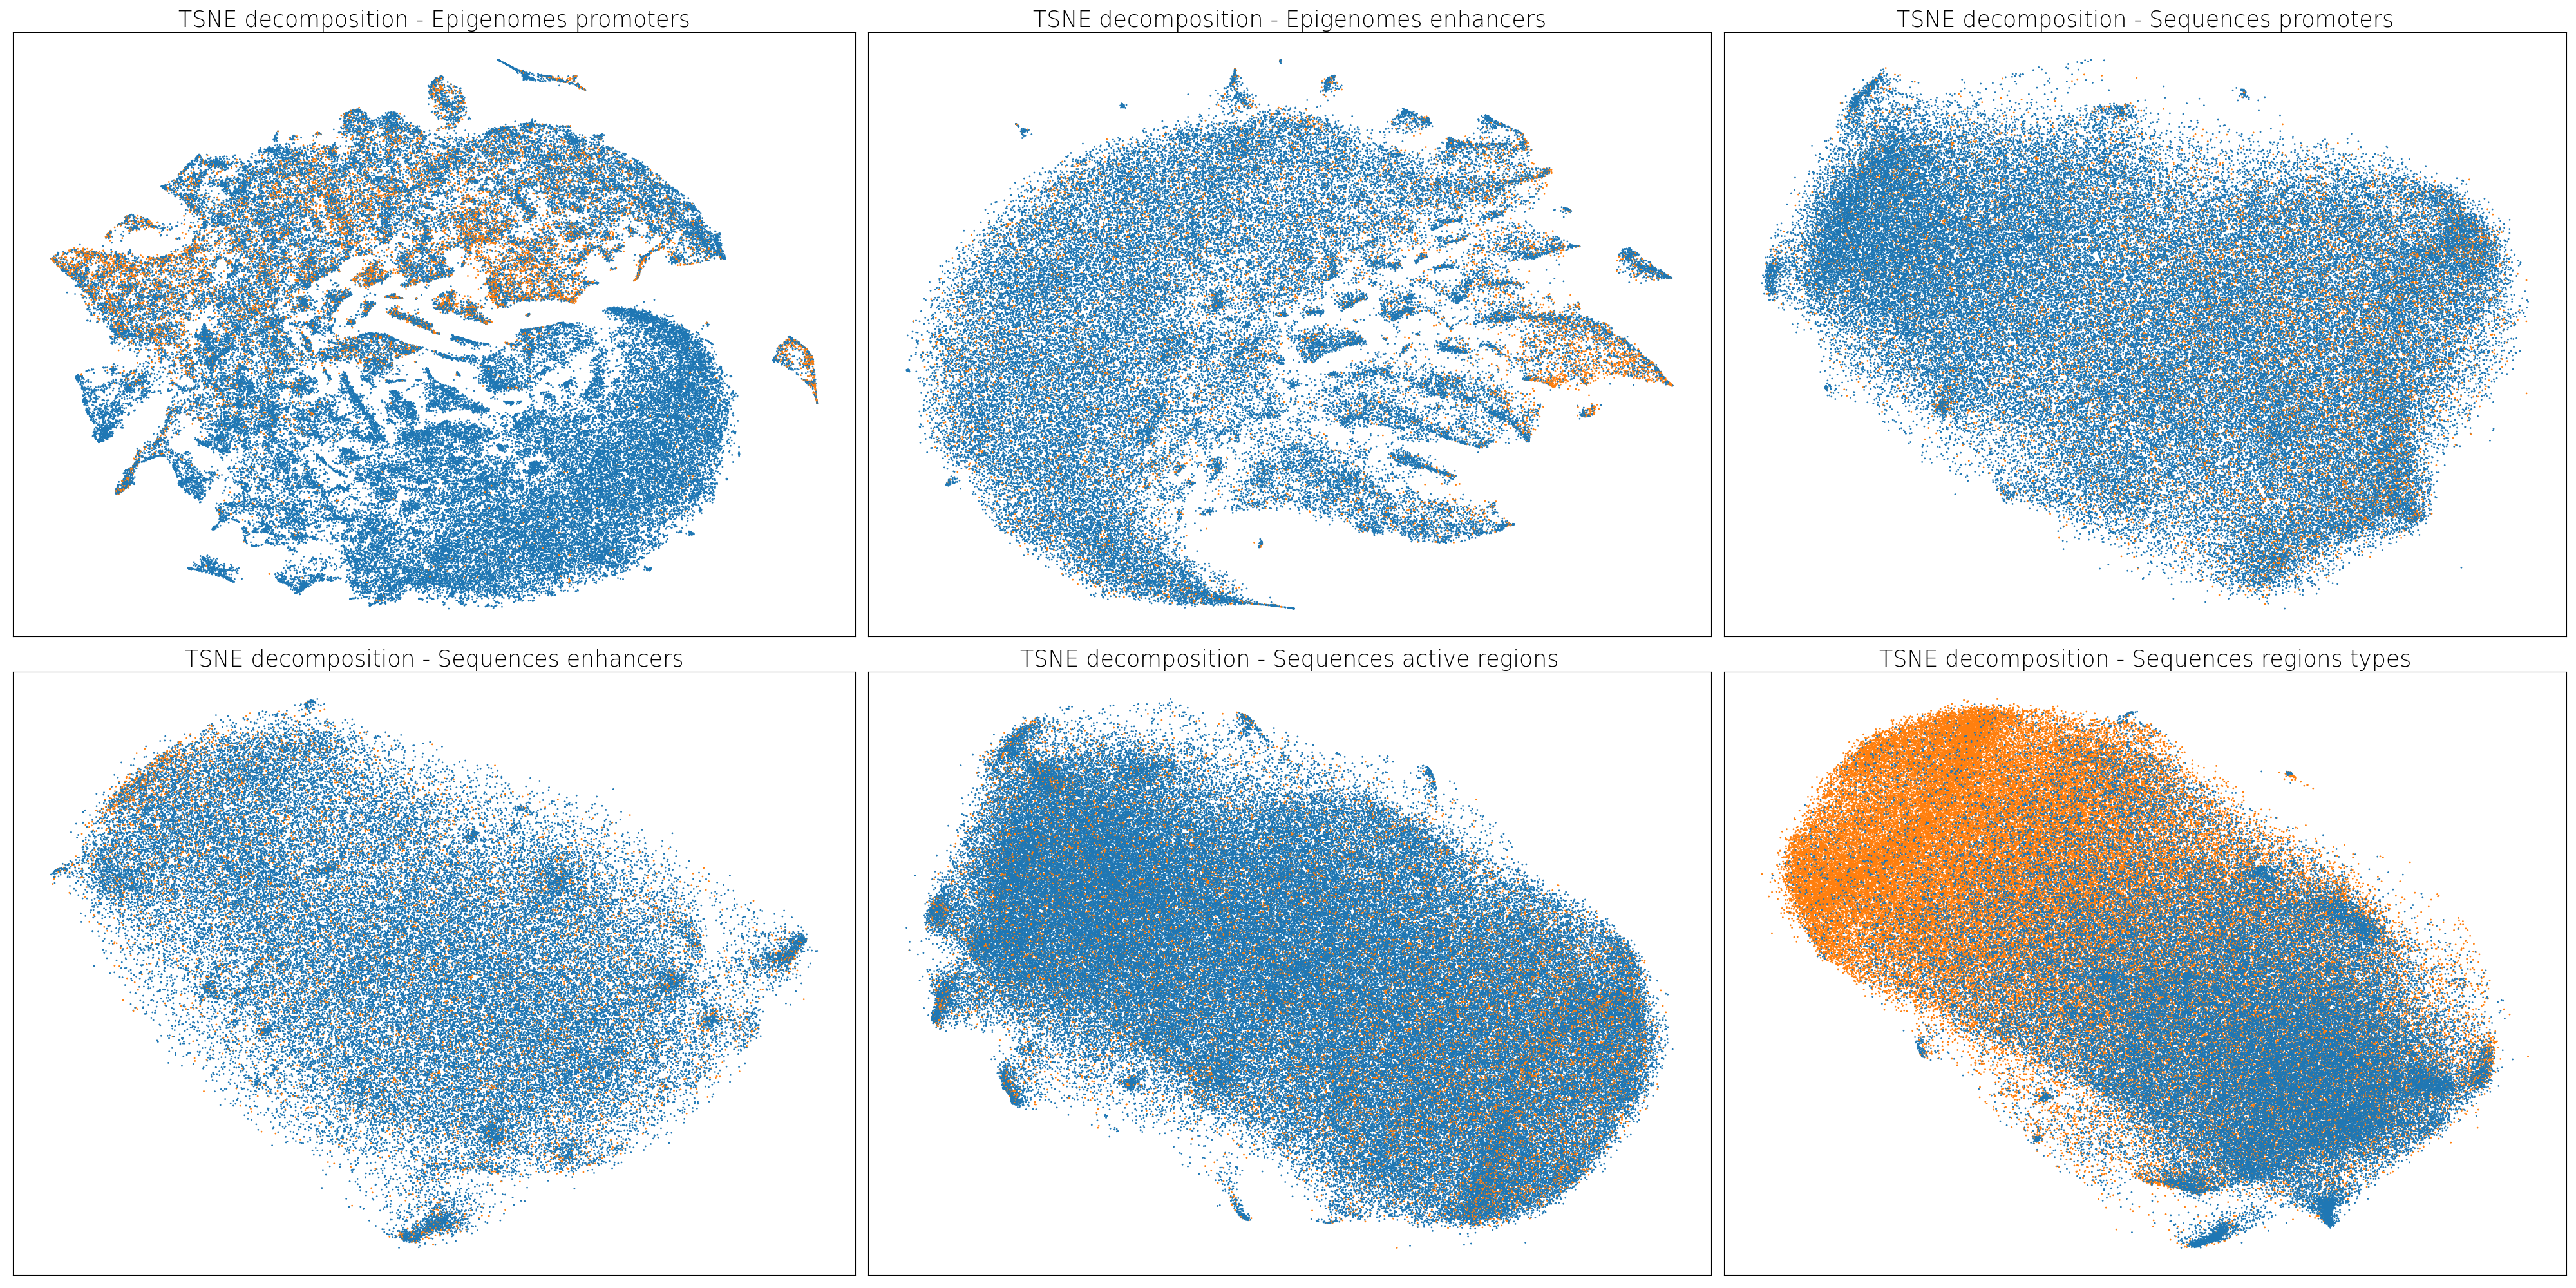
\includegraphics[width=0.95\linewidth]{../images/tsne_5000.png}
\caption{TSNE data decomposition}
\end{figure}
\newpage
\subsection{Feature selection}

Since the epigenomic data has a large number of feature, it is important
to apply methods to find those features which are unnecessary or
dangerous for the learning machines and to remove them. Only he
epigenomic data are treated using this procedure, while the sequence
data are used as is. In this project, three different types of feature
selection techniques are used:

\begin{itemize}
\item
  \textbf{Check of feature-output correlation:} the feature not
  correlated with output can be removed. In particular, the Person and
  Spearman methods are used to finding monotonic and linear correlation
  respectively and, subsequently, the uncorrelated features found using
  these methods are tested with the MIC algorithm to check non-linear
  correlation with output. In the end, those features whit no
  correlation with output (bot linear and non-linear) are removed. 
\item
  \textbf{Check of feature-feature correlation:} the pairs of feature
  strongly correlated are not necessary for the learning machine,
  because they express the "same concept". In this way, in a pair of
  correlated features, the one with less entropy can be removed. In this
  project are applied the Pearson and Spearman method to check
  feature-feature monotonic correlation.
\item
  \textbf{Automatic feature selection:} the last way to remove feature
  is to test their utility for a learning machine. In particular, The
  Boruta method with a random forest is applied to the data and those
  features useless for that model have been dropped.
\end{itemize}

All these techniques are applied. The initial amount of features is 207
for promoters and enhancers. More in detail, the following pipeline is
applied for feature selection:

\begin{itemize}
\item
  Apply the Pearson method for feature-output correlation. There are
  selected 9 uncorrelated features for promoters and 28 for enhancers
  with a p\_value threshold of 0.01
\item
  Apply the Spearman method for feature-output correlation. There are
  selected 6 uncorrelated features for promoters and 27 for enhancers
  with a p\_value threshold of 0.01
\item
  The uncorrelated features found with Pearson and Spearman are not
  unique, so the two sets are unified with no repetition. The resulting
  set has 12 and 32 features for promoters and enhancers respectively
\item
  Apply the MIC method for feature-output correlation on the feature
  selected with Pearson and Spearman to check the non-linear
  correlation. After the execution, MIC find no non-linear correlation
  on the examined features with a threshold of 0.05, so there are
  removed 12 features for promoters and 32 for enhancers
\item
  Apply the Pearson method to find the feature-feature correlation. In
  this case, there are selected 0 pair of extremely correlated features
  using a p\_value threshold of 0.01 and a correlation threshold of
  0.95, so no features are removed
\item
  Apply the Spearman method to find the feature-feature correlation. In
  this case, there are selected 0 pair of extremely correlated features
  using a p\_value threshold of 0.01 and a correlation threshold of
  0.95, so no features are removed
\item
  Apply the Boruta method to remove the features useless for the random
  forest. The random forest classifier is set using the following
  parameters:

  \begin{itemize}
  \item
    n\_estimators = auto
  \item
    alpha = 0.05
  \item
    max\_iter = 10
  \item
    random\_state = 42
  \end{itemize}
\item
  After 300 iterations Boruta finds 4 useless features for promoters and
  36 for enhancers.
\item
  In the end, the total amount of features is 191 and 139 for promoters
  and enhancers respectively. In the following subsections, the features
  selection techniques are explained more in detail. 
\end{itemize}

\subsubsection{Data correlation with output}

A check which can be applied to the data is the correlation between
features and output. If a feature isn't correlated with a specific
output it is completely useless and it can be dropped. To do this, the
Pearson and Spearman tests are applied, which measure the monotonic and
linear correlations respectively. After that, the candidate
non-correlated features are tested with the MIC (Maximal information
coefficient) that tests the non-linear correlation between features and
output. Only the features found with Pearson and Spearman methods are
tested using MIC to check if they nave non-linear correlation with
output. More in detail, the Pearson correlation method measures the
linear correlation between the two datasets. In particular, the Pearson
coefficient has a value between -1 and +1, where -1 is a total negative
linear correlation, 0 implying no correlation, and +1 is a total
positive linear correlation. Instead, the Spearman correlation
coefficient doesn't require that the two datasets are normalized and it
measures the monotonicity relationship between them. The Spearman
coefficient varies between -1 and +1, like Pearson's. Now is the moment
to apply the MIC procedures to the feature selected by Pearson and
Spearman method in order to find non-linear correlations. It is
important to specify that Pearson's, Spearman's and MIC's results are
significant if they are is calculated over a large dataset, typically
with 500 samples or more. In the end, the features uncorrelated with
output can be removed.

\subsubsection{Feature correlation}

To make the data less heavy, it is possible to find and remove tightly
correlated features. The correlation can be measured using the Pearson
or MIC method. In this project, the Pearson method is used to save time
(MIC is computationally complex). When two features appear correlated,
the one with the lower entropy is removed. The entropy can be
interpreted as the average level of information or uncertainty given by
a variable. In this project, there aren't features extremely correlated
but it is interesting to examine the most correlated and least
correlated features, as shown in the images below. The first pair of
images show the most correlated and uncorrelated features in promoters
and enhancers respectively found with Pearson method. The last pair
show the two most correlated and uncorrelated features found with
Spearman method. The blue and orange colors refers to inactive and
active region respectively.

\begin{figure}[h!]
\centering
\includegraphics[width=0.98\linewidth]{../images/plot_pearson_promoters_correlated_uncorrelated.png}
\caption{Most correlated and uncorrelated feature with output for promoters found with Pearson method}
\end{figure}
\newpage
\begin{figure}[h!]
\centering
\includegraphics[width=0.98\linewidth]{../images/plot_pearson_enhancers_correlated_uncorrelated.png}
\caption{Most correlated and uncorrelated feature with output for enhancers found with Pearson method}
\end{figure}

\begin{figure}[h!]
\centering
\includegraphics[width=0.98\linewidth]{../images/plot_spearman_promoters_correlated_uncorrelated.png}
\caption{Most correlated and uncorrelated feature with output for promoters found with Spearman method}
\end{figure}
\newpage
\begin{figure}[h!]
\centering
\includegraphics[width=0.98\linewidth]{../images/plot_spearman_enhancers_correlated_uncorrelated.png}
\caption{Most correlated and uncorrelated feature with output for enhancers found with Spearman method}
\end{figure}

\subsubsection{Automatic feature selection: the Boruta
method}

The feature selection is the process of finding the relevant features to
use for learning a model. Indeed the data may have some irrelevant or
redundant features, which can be removed without information loss to
make the learning process easier. Until now the feature selection
process was done using manual methods, based on the feature to feature
and the feature to output correlation. These methods are certainly
effective but there are not enough: the features are considered one or
to at a time to find a linear or non-linear correlation between the
output or another feature. Boruta, an automatic method for feature
selection, considers the features as a whole and use a specific
classification algorithm to find the irrelevant features. Boruta is a
wrapper built around the random forest algorithm, chosen because it is
relatively quick to compute and it usually can run without parameters
specification. In fact, Boruta is an ensemble method in which
classification is performed by voting of multiple decision trees, each
of them is independently developed on different samples of the training
set. The importance measure of an attribute is the loss of accuracy of
classification, caused by random permutation of this attribute values in
the various trees.

\subsection{Experiments evaluation}

After preprocessing and feature selection, the data are ready to pass to
the learning models. The holdout technique is used for testing the
models. This method consists into split the dataset in two separate
sets: the training set (used to train the leaning machine to learn) and
the test set (used to test the model performances). In this case, the
split is 80\% and 20\% for training and test set. The experiments are
executed over multiple holdouts, 50 for epigenomic data, and 3 for
sequence data, to make the models' evaluation more robust. In
particular, the StratifiedShuffleSplit of sklearn is used to make the
holdouts. This method randomly separates the training and test set
indices, preserving the percentage of samples for each class. It is set
with 42 as random\_state parameter.

The metrics used to evaluate the models are the following:

\begin{itemize}
	\item
	\textbf{accuracy:} is the ration between the correct predictions and
	the total number of samples.
	\item
	\textbf{auPRC}: the area under the precision-recall curve is a useful
	measure of success of prediction when the classes are imbalanced. The
	precision-recall curve shows the tradeoff between precision and recall
	of different thresholds. A high area under the curve represents both
	high recall and high precision, where high precision relates to a low
	false-positive rate, and high recall relates to a low false-negative
	rate. The auPRC value is between 0 and 1 and a high value denotes a
	good predictor.
	\item
	\textbf{auROC}: the area under receiver operating characteristic is a
	metric specific for binary classification tasks. It indicates the
	fraction between the true positive rate and the false-positive rates.
	Differently, form auPRC, its values are between 0.5 and 1.
\end{itemize}

Each metric is calculated for each model the final results are the mean
and the standard deviation obtained through the various holdouts. These
results are finally compared using the Wilcoxon signed-rank test with a
p\_value threshold of 0.01. It is a non-parametric statistical test to
compare hypotheses made on repeated measures.

\section{Experimental results}

\subsection{Epigenomic experiments}

\subsubsection{Promoters}

In this section are reported the experiment results for active vs
inactive promoters task using epigenomic data. For each metric there are
a table and a plot to confront the learning machine performance.
\newpage
\textbf{Accuracy}

\begin{longtable}[]{@{}lll@{}}
\toprule
\textbf{Models} & \textbf{Training} & \textbf{Test}\tabularnewline
\midrule
\endhead
DecisionTree & mean = 0.7241 & mean = 0.7148\tabularnewline
& STD = 0.0124 & STD = 0.0123\tabularnewline
RandomForest & mean = 0.7522 & mean = 0.7408\tabularnewline
& STD = 0.0014 & STD = 0.0022\tabularnewline
Perceptron & mean = 0.883 & mean = 0.882\tabularnewline
& STD = 0.0005 & STD = 0.0015\tabularnewline
MLP & mean = 0.9638 & mean = 0.8621\tabularnewline
& STD = 0.0041 & STD = 0.0057\tabularnewline
FFNN\_1 & mean = 0.956 & mean = 0.8634\tabularnewline
& STD = 0.0023 & STD = 0.0037\tabularnewline
FFNN\_2 & mean = 0.885 & mean = 0.8848\tabularnewline
& STD = 0.0002 & STD = 0.0002\tabularnewline
FFNN\_3 & mean = 0.8895 & mean = 0.8854\tabularnewline
& STD = 0.0038 & STD = 0.0007\tabularnewline
FFNN\_4 & mean = 0.8886 & mean = 0.884\tabularnewline
& STD = 0.0007 & STD = 0.0011\tabularnewline
\bottomrule
\end{longtable}

\begin{figure}[h!]
\centering
\includegraphics[width=0.77\linewidth]{../images/epigemomic_results/promoters/accuracy.png}
\caption{Accuracy metric for promoters epigenomic experiments}
\end{figure}

\textbf{AUROC}

\begin{longtable}[]{@{}lll@{}}
\toprule
\textbf{Models} & \textbf{Training} & \textbf{Test}\tabularnewline
\midrule
\endhead
DecisionTree & mean = 0.8081 & mean = 0.7862\tabularnewline
& STD = 0.0019 & STD = 0.0033\tabularnewline
RandomForest & mean = 0.8384 & mean = 0.8117\tabularnewline
& STD = 0.0008 & STD = 0.0027\tabularnewline
Perceptron & mean = 0.8674 & mean = 0.8638\tabularnewline
& STD = 0.0008 & STD = 0.0026\tabularnewline
MLP & mean = 0.9813 & mean = 0.8433\tabularnewline
& STD = 0.0014 & STD = 0.0054\tabularnewline
FFNN\_1 & mean = 0.9774 & mean = 0.8392\tabularnewline
& STD = 0.0016 & STD = 0.0057\tabularnewline
FFNN\_2 & mean = 0.9184 & mean = 0.8766\tabularnewline
& STD = 0.0039 & STD = 0.0028\tabularnewline
FFNN\_3 & mean = 0.9015 & mean = 0.8733\tabularnewline
& STD = 0.0103 & STD = 0.0042\tabularnewline
FFNN\_4 & mean = 0.8893 & mean = 0.8727\tabularnewline
& STD = 0.001 & STD = 0.0025\tabularnewline
\bottomrule
\end{longtable}

\begin{figure}[h!]
\centering
\includegraphics[width=0.77\linewidth]{../images/epigemomic_results/promoters/auroc.png}
\caption{AUROC metric for promoters epigenomic experiments}
\end{figure}

\textbf{AUPRC}

\begin{longtable}[]{@{}lll@{}}
\toprule
\textbf{Models} & \textbf{Training} & \textbf{Test}\tabularnewline
\midrule
\endhead
DecisionTree & mean = 0.2703 & mean = 0.2531\tabularnewline
& STD = 0.0046 & STD = 0.0037\tabularnewline
RandomForest & mean = 0.3018 & mean = 0.2784\tabularnewline
& STD = 0.0011 & STD = 0.0023\tabularnewline
Perceptron & mean = 0.3953 & mean = 0.3867\tabularnewline
& STD = 0.0022 & STD = 0.0077\tabularnewline
MLP & mean = 0.8998 & mean = 0.3524\tabularnewline
& STD = 0.0089 & STD = 0.011\tabularnewline
FFNN\_1 & mean = 0.878 & mean = 0.3459\tabularnewline
& STD = 0.0082 & STD = 0.0082\tabularnewline
FFNN\_2 & mean = 0.496 & mean = 0.4245\tabularnewline
& STD = 0.0145 & STD = 0.009\tabularnewline
FFNN\_3 & mean = 0.5009 & mean = 0.4146\tabularnewline
& STD = 0.0384 & STD = 0.0092\tabularnewline
FFNN\_4 & mean = 0.4632 & mean = 0.4047\tabularnewline
& STD = 0.0053 & STD = 0.0076\tabularnewline
\bottomrule
\end{longtable}

\begin{figure}[h!]
\centering
\includegraphics[width=0.77\linewidth]{../images/epigemomic_results/promoters/auprc.png}
\caption{AUPRC metric for promoters epigenomic experiments}
\end{figure}

\subsubsection{Enhancers}

In this section are reported the experiment results for active vs
inactive enhancers task using epigenomic data. For each metric there are
a table and a plot to confront the learning machine performance.

\textbf{Accuracy}

\begin{longtable}[]{@{}lll@{}}
	\toprule
	\textbf{Models} & \textbf{Training} & \textbf{Test}\tabularnewline
	\midrule
	\endhead
	DecisionTree & mean = 0.7417 & mean = 0.7316\tabularnewline
	& STD = 0.0303 & STD = 0.0297\tabularnewline
	RandomForest & mean = 0.8248 & mean = 0.8144\tabularnewline
	& STD = 0.0023 & STD = 0.0037\tabularnewline
	Perceptron & mean = 0.8978 & mean = 0.897\tabularnewline
	& STD = 0.0003 & STD = 0.0009\tabularnewline
	MLP & mean = 0.9793 & mean = 0.8545\tabularnewline
	& STD = 0.0142 & STD = 0.0108\tabularnewline
	FFNN\_1 & mean = 0.9784 & mean = 0.8501\tabularnewline
	& STD = 0.0014 & STD = 0.0046\tabularnewline
	FFNN\_2 & mean = 0.8964 & mean = 0.8958\tabularnewline
	& STD = 0.0012 & STD = 0.0009\tabularnewline
	FFNN\_3 & mean = 0.8991 & mean = 0.8971\tabularnewline
	& STD = 0.0015 & STD = 0.0009\tabularnewline
	FFNN\_4 & mean = 0.9021 & mean = 0.8978\tabularnewline
	& STD = 0.0004 & STD = 0.001\tabularnewline
	\bottomrule
\end{longtable}

\begin{figure}[h!]
	\centering
	\includegraphics[width=0.6\linewidth]{../images/epigemomic_results/enhancers/accuracy.png}
	\caption{Accuracy metric for enhancers epigenomic experiments}
\end{figure}

\textbf{AUROC}

\begin{longtable}[]{@{}lll@{}}
	\toprule
	\textbf{Models} & \textbf{Training} & \textbf{Test}\tabularnewline
	\midrule
	\endhead
	DecisionTree & mean = 0.6453 & mean = 0.6168\tabularnewline
	& STD = 0.0029 & STD = 0.0067\tabularnewline
	RandomForest & mean = 0.6521 & mean = 0.626\tabularnewline
	& STD = 0.0017 & STD = 0.006\tabularnewline
	Perceptron & mean = 0.6903 & mean = 0.6796\tabularnewline
	& STD = 0.002 & STD = 0.0071\tabularnewline
	MLP & mean = 0.9608 & mean = 0.6097\tabularnewline
	& STD = 0.0263 & STD = 0.0109\tabularnewline
	FFNN\_1 & mean = 0.9652 & mean = 0.6136\tabularnewline
	& STD = 0.0017 & STD = 0.0083\tabularnewline
	FFNN\_2 & mean = 0.8646 & mean = 0.6703\tabularnewline
	& STD = 0.0124 & STD = 0.008\tabularnewline
	FFNN\_3 & mean = 0.7462 & mean = 0.6833\tabularnewline
	& STD = 0.0206 & STD = 0.0062\tabularnewline
	FFNN\_4 & mean = 0.7284 & mean = 0.6816\tabularnewline
	& STD = 0.0027 & STD = 0.0068\tabularnewline
	\bottomrule
\end{longtable}

\begin{figure}[h!]
	\centering
	\includegraphics[width=0.77\linewidth]{../images/epigemomic_results/enhancers/auroc.png}
	\caption{AUROC metric for enhancers epigenomic experiments}
\end{figure}

\textbf{AUPRC}

\begin{longtable}[]{@{}lll@{}}
	\toprule
	\textbf{Models} & \textbf{Training} & \textbf{Test}\tabularnewline
	\midrule
	\endhead
	DecisionTree & mean = 0.1617 & mean = 0.1464\tabularnewline
	& STD = 0.0045 & STD = 0.004\tabularnewline
	RandomForest & mean = 0.184 & mean = 0.1636\tabularnewline
	& STD = 0.0012 & STD = 0.004\tabularnewline
	Perceptron & mean = 0.2964 & mean = 0.2852\tabularnewline
	& STD = 0.0029 & STD = 0.0103\tabularnewline
	MLP & mean = 0.9059 & mean = 0.1867\tabularnewline
	& STD = 0.0803 & STD = 0.0137\tabularnewline
	FFNN\_1 & mean = 0.9187 & mean = 0.1726\tabularnewline
	& STD = 0.0039 & STD = 0.0088\tabularnewline
	FFNN\_2 & mean = 0.452 & mean = 0.2824\tabularnewline
	& STD = 0.0255 & STD = 0.0118\tabularnewline
	FFNN\_3 & mean = 0.3494 & mean = 0.2901\tabularnewline
	& STD = 0.0202 & STD = 0.0116\tabularnewline
	FFNN\_4 & mean = 0.3558 & mean = 0.2858\tabularnewline
	& STD = 0.0042 & STD = 0.011\tabularnewline
	\bottomrule
\end{longtable}

\begin{figure}[h!]
	\centering
	\includegraphics[width=0.77\linewidth]{../images/epigemomic_results/enhancers/auprc.png}
	\caption{AUPRC metric for enhancers epigenomic experiments}
\end{figure}
\subsubsection{Observations}
\paragraph{Promoters' obervations}
The following observations refer to the experiments executed on the promoters' epigenomic data.
\newline
\par
\emph{1) DecisionTree and RandomForest perform worst than other models.}
The results show that DecisionTree and Random Forest perform worst than
the other models according to all metrics, both for promoters and
enhancers.

\emph{2) There is a big problem of overfitting with complex deep
networks.} The data decomposition graphs show that the promoters'
epigenomic data are not clearly separable and the complex models tend to
learn data without generalizing. This happens in particular with the MLP
and FFNN\_1 and it is visible in the AUPRC metric.

\emph{3) The perceptron performance is comparable with more complex
models.} This model indeed does not overfit because of its very simple
structure and it can better generalize. In particular, according to the
Wilcoxon test, the perceptron performs better than DecisionTree,
RandomForest, MLP, and FFNN\_1 in all metrics.

\emph{4) The FFNN\_3 does not improve the performance despite it tries to
resolve the class imbalance problem.} The measures adopted have only
prevented overfitting but the test result is not the best. Besides,
FFNN\_3 has the largest STD in the training results according to all
metrics.

\emph{5) FFNN\_2 is the best model.} According to the Wilcoxon test,
this model performs better than the others in all metrics, except for
the FFNN\_3 according to the accuracy. This model has a complex
architecture, composed of 5 hidden layers and a big dropout for each of
them. This strategy allows the network to learn the data without
overfitting.

\emph{6) All models fail to recognize the positive samples.} The
accuracy and AUROC are high and they hide the real model performances.
This is because the dataset is unbalanced (the positive samples
represent the minority class) and these metrics do not capture the fact
that the model correctly classifies only a few part of the positive
samples. Thanks to the AUPRC, it is evident that the models produce a
lot of false-negative because this metric is always less than 0.5.
\newline
\paragraph{Enhancers' obervations}
The following observations refer to the experiments executed on the enhancers' epigenomic data.
\newline
\par
\emph{1) DecisionTree and RandomForest perform worst than other models.}
The results show that DecisionTree and Random Forest perform worst than
the other models according to all metrics, both for promoters and
enhancers.

\emph{2) The overfitting problem is more pronounced than promoters.} The
data decomposition graphs show that the enhancers' epigenomic data are
not clearly separable and the complex models tend to learn data without
generalizing. This happens in particular with the MLP and FFNN\_1 and it
is visible in the AUPRC metric.

\emph{3) The perceptron performance is comparable with more complex
models.} This model indeed does not overfit because of its very simple
structure and it can better generalize. In particular, according to the
Wilcoxon test, the perceptron performs better than DecisionTree,
RandomForest, MLP, and FFNN\_1. Also, the FFNN\_2 is worst than
perceptron according to accuracy and AUROC, while for AUPRC these two
models are statistically identical.

\emph{4) The reduction of overfitting does not improve performance.}
Unlike promoters' experiments, the networks are not able to better
generalize despite the reduction of the training metrics values. The
enhancers' epigenomic data are less separable than promoters' ones, as
shown by PCA and TSNE data decomposition graphs. Moreover, the enhancers
have fewer samples than the promoters and the data imbalance is more
pronounced.

\emph{5) There isn't the best model.} The deep networks tested for
enhancers win and loose according to various metrics. For accuracy, the
best model is the FFNN\_4. Despite according to the AUROC, the
models that perform better are FFNN\_3 and FFNN\_4: they are
statistically identical. Finally, for AUPRC, the FFNN\_3 is the best
model.
\newpage
\subsection{Sequence experiments}

\subsubsection{Promoters}

\textbf{Accuracy}

\begin{longtable}[]{@{}lll@{}}
\toprule
\textbf{Models} & \textbf{Training} & \textbf{Test}\tabularnewline
\midrule
\endhead
Perceptron & mean = 0.8848 & mean = 0.8847\tabularnewline
& STD = 0.0 & STD = 0.0\tabularnewline
MLP & mean = 0.983 & mean = 0.8\tabularnewline
& STD = 0.0132 & STD = 0.0071\tabularnewline
FFNN\_1 & mean = 0.9984 & mean = 0.8188\tabularnewline
& STD = 0.0001 & STD = 0.0006\tabularnewline
CNN\_1 & mean = 0.9719 & mean = 0.8381\tabularnewline
& STD = 0.0008 & STD = 0.0017\tabularnewline
CNN\_2 & mean = 0.9918 & mean = 0.807\tabularnewline
& STD = 0.0021 & STD = 0.0187\tabularnewline
CNN\_3 & mean = 0.956 & mean = 0.8641\tabularnewline
& STD = 0.0504 & STD = 0.0146\tabularnewline
\bottomrule
\end{longtable}

\begin{figure}[h!]
\centering
\includegraphics[width=0.8\linewidth]{../images/sequence_results/promoters/accuracy.png}
\caption{Accuracy metric for promoters sequence experiments}
\end{figure}

\textbf{AUROC}

\begin{longtable}[]{@{}lll@{}}
\toprule
\textbf{Models} & \textbf{Training} & \textbf{Test}\tabularnewline
\midrule
\endhead
Perceptron & mean = 0.5622 & mean = 0.5031\tabularnewline
& STD = 0.0027 & STD = 0.0024\tabularnewline
MLP & mean = 0.9933 & mean = 0.5049\tabularnewline
& STD = 0.0079 & STD = 0.005\tabularnewline
FFNN\_1 & mean = 0.9998 & mean = 0.5039\tabularnewline
& STD = 0.0 & STD = 0.003\tabularnewline
CNN\_1 & mean = 0.9893 & mean = 0.4914\tabularnewline
& STD = 0.0008 & STD = 0.0076\tabularnewline
CNN\_2 & mean = 0.9973 & mean = 0.5003\tabularnewline
& STD = 0.0006 & STD = 0.0052\tabularnewline
CNN\_3 & mean = 0.8313 & mean = 0.5006\tabularnewline
& STD = 0.2349 & STD = 0.0035\tabularnewline
\bottomrule
\end{longtable}

\begin{figure}[h!]
\centering
\includegraphics[width=0.8\linewidth]{../images/sequence_results/promoters/auroc.png}
\caption{AUROC metric for promoters sequence experiments}
\end{figure}
\newpage
\textbf{AUPRC}

\begin{longtable}[]{@{}lll@{}}
\toprule
\textbf{Models} & \textbf{Training} & \textbf{Test}\tabularnewline
\midrule
\endhead
Perceptron & mean = 0.14 & mean = 0.116\tabularnewline
& STD = 0.0026 & STD = 0.0013\tabularnewline
MLP & mean = 0.9697 & mean = 0.1176\tabularnewline
& STD = 0.0345 & STD = 0.0014\tabularnewline
FFNN\_1 & mean = 0.9991 & mean = 0.1175\tabularnewline
& STD = 0.0001 & STD = 0.001\tabularnewline
CNN\_1 & mean = 0.9472 & mean = 0.1126\tabularnewline
& STD = 0.0031 & STD = 0.0026\tabularnewline
CNN\_2 & mean = 0.9843 & mean = 0.1155\tabularnewline
& STD = 0.0025 & STD = 0.0017\tabularnewline
CNN\_3 & mean = 0.6925 & mean = 0.1153\tabularnewline
& STD = 0.4083 & STD = 0.0012\tabularnewline
\bottomrule
\end{longtable}

\begin{figure}[h!]
\centering
\includegraphics[width=0.8\linewidth]{../images/sequence_results/promoters/auprc.png}
\caption{AUPRC metric for promoters sequence experiments}
\end{figure}

\subsubsection{Enhancers}\label{header-n1661}

\textbf{Accuracy}

\begin{longtable}[]{@{}lll@{}}
\toprule
\textbf{Models} & \textbf{Training} & \textbf{Test}\tabularnewline
\midrule
\endhead
Perceptron & mean = 0.8937 & mean = 0.8938\tabularnewline
& STD = 0.0 & STD = 0.0\tabularnewline
MLP & mean = 1.0 & mean = 0.8245\tabularnewline
& STD = 0.0 & STD = 0.0022\tabularnewline
FFNN\_1 & mean = 0.9991 & mean = 0.8424\tabularnewline
& STD = 0.0006 & STD = 0.0033\tabularnewline
CNN\_1 & mean = 0.987 & mean = 0.8504\tabularnewline
& STD = 0.0013 & STD = 0.0175\tabularnewline
CNN\_2 & mean = 0.9916 & mean = 0.8146\tabularnewline
& STD = 0.0047 & STD = 0.0489\tabularnewline
CNN\_3 & mean = 0.9948 & mean = 0.8667\tabularnewline
& STD = 0.0001 & STD = 0.0028\tabularnewline
\bottomrule
\end{longtable}

\begin{figure}[h!]
\centering
\includegraphics[width=0.82\linewidth]{../images/sequence_results/enhancers/accuracy.png}
\caption{Accuracy metric for enhancers sequence experiments}
\end{figure}
\newpage
\textbf{AUROC}

\begin{longtable}[]{@{}lll@{}}
\toprule
\textbf{Models} & \textbf{Training} & \textbf{Test}\tabularnewline
\midrule
\endhead
Perceptron & mean = 0.5865 & mean = 0.5017\tabularnewline
& STD = 0.0012 & STD = 0.0032\tabularnewline
MLP & mean = 1.0 & mean = 0.4973\tabularnewline
& STD = 0.0 & STD = 0.0047\tabularnewline
FFNN\_1 & mean = 0.9999 & mean = 0.4976\tabularnewline
& STD = 0.0 & STD = 0.0026\tabularnewline
CNN\_1 & mean = 0.9969 & mean = 0.5071\tabularnewline
& STD = 0.0006 & STD = 0.0008\tabularnewline
CNN\_2 & mean = 0.9966 & mean = 0.4949\tabularnewline
& STD = 0.0022 & STD = 0.0028\tabularnewline
CNN\_3 & mean = 0.9988 & mean = 0.4976\tabularnewline
& STD = 0.0002 & STD = 0.0023\tabularnewline
\bottomrule
\end{longtable}

\begin{figure}[h!]
\centering
\includegraphics[width=0.8\linewidth]{../images/sequence_results/enhancers/auroc.png}
\caption{AUROC metric for enhancers sequence experiments}
\end{figure}
\newpage
\textbf{AUPRC}

\begin{longtable}[]{@{}lll@{}}
\toprule
\textbf{Models} & \textbf{Training} & \textbf{Test}\tabularnewline
\midrule
\endhead
Perceptron & mean = 0.1413 & mean = 0.1068\tabularnewline
& STD = 0.0013 & STD = 0.0017\tabularnewline
MLP & mean = 1.0 & mean = 0.1046\tabularnewline
& STD = 0.0 & STD = 0.0023\tabularnewline
FFNN\_1 & mean = 0.9997 & mean = 0.1046\tabularnewline
& STD = 0.0002 & STD = 0.0008\tabularnewline
CNN\_1 & mean = 0.9831 & mean = 0.1076\tabularnewline
& STD = 0.0028 & STD = 0.0001\tabularnewline
CNN\_2 & mean = 0.9839 & mean = 0.1041\tabularnewline
& STD = 0.0112 & STD = 0.0015\tabularnewline
CNN\_3 & mean = 0.9906 & mean = 0.1051\tabularnewline
& STD = 0.0015 & STD = 0.0012\tabularnewline
\bottomrule
\end{longtable}

\begin{figure}[h!]
\centering
\includegraphics[width=0.8\linewidth]{../images/sequence_results/enhancers/auprc.png}
\caption{AUPRC metric for enhancers sequence experiments}
\end{figure}

\subsubsection{Observations}\label{header-n1829}

\emph{1) The sequence data are insufficient to execute all the tasks.}
The accuracy metrics show that the models have good performances but the
AUPRC and AUROC metrics reveal the opposite, both for promoters and
enhancers. In particular, the AUROC is closed to its minimum values in
all experiments, like the AUPRC. This means that the models return
casual values. These results are confirmed by the data decomposition
graphs, that highlight a total data inseparability. The CNNs, which
should learn automatically the hidden features of the data, can't
improve the performances.

\emph{2) The overfitting problem has not been resolved.} The AUPRC and
AUROC metrics show that the models are not able to generalize and the
high value of accuracy is caused by the data imbalance.

\section{Conclusions}

Using the HEK293 cell line, the experiments results, validated with the
Wilcoxon tests, shows that the feed-forward neural networks can
predict the active and inactive regulatory region using epigenomic data more accurately than the other models using the epigenomic data. However, given the data
complexity, this is true if the networks prevent the overfitting,
otherwise the models aren't able to generalize. This is confirmed by the
perceptron's results, which works similarly to more complex networks.
Despite this, observing the ARPC, it is clear that the task remains difficult. This metric is low compared to the others and it means a low AUPRC means that the models fail to recognize the positive samples. 
For enhancers this fact is particularly pronounced.
In general, the experiments on the epigenomic data show that on HEK293 cell line the deep networks perform well only if their architecture is extremely simple (as in the case of the perceptron). For more complex models it is necessary to adopt aggressive techniques to prevent overfitting.
Instead using the sequence data, the tasks to determine active and
inactive regulatory region do not obtain good results. The models,
including the CNNs, aren't able to learn the complex distribution of
data. These results are confirmed by the data decomposition graphs, which show the total overlap of the active and inactive regulatory region sequence data.
\newpage
\begin{thebibliography}{99}

\bibitem{}
Yifeng Li, Wenqiang Shi, and Wyeth W. Wasserman. \textit{"Genome-wide
prediction of cis-regulatory regions using supervised deep learning
methods"}

\bibitem{}
Xu Min, Wanwen Zeng, Shengquan Chen, Ning Chen, Ting Chen, Rui Jiang \textit{"Predicting enhancers with deep convolutional
neural networks"}

\bibitem{}
Kelley DR, Snoek J, Rinn JL. 2016. \textit{Basset: learning the
regulatory code of the accessible genome with deep convolutional neural
networks.}

\bibitem{}
 David R. Kelley, Yakir A. Reshef, Maxwell Bileschi, David
Belanger, Cory Y. McLean, and Jasper Snoek. \textit{"Sequential regulatory
activity prediction across chromosomes with convolutional neural
networks"}

\bibitem{}
Luca Cappelletti, Alessandro Petrini, Jessica Gliozzo, Elena
Casiraghi, Max Schubach, Martin Kircher, Giorgio Valentini. \textit{"Bayesian
optimization improves tissue-specific prediction of active regulatory
regions with deep neural networks"}

\end{thebibliography}


\end{document}